\documentclass[12pt,prb,aps,epsf]{report}
\usepackage[utf8]{inputenc}
\usepackage{amsmath}
\usepackage{amsfonts}
\usepackage{amssymb}
\usepackage{graphicx} 
\usepackage{latexsym} 
\usepackage[toc,page]{appendix}
\usepackage{listings}
\usepackage{xcolor}
\usepackage{soul}
\usepackage[T1]{fontenc}
\usepackage{amsthm}
\usepackage{mathtools}
\usepackage{setspace}
\usepackage{array,multirow,makecell}
\usepackage{geometry}
\usepackage{textcomp}
\usepackage{float}
%\usepackage{siunitx}
\usepackage{cancel}
%\usepackage{tikz}
%\usetikzlibrary{calc, shapes, backgrounds, arrows, decorations.pathmorphing, positioning, fit, petri, tikzmark}
\usepackage{here}
\usepackage{titlesec}
%\usepackage{bm}
\usepackage{bbold}

\geometry{hmargin=2cm,vmargin=2cm}

\begin{document}
	
	\title{MP 08 Interférences lumineuses}
	\author{Hugo}
	
	\maketitle
	
	\tableofcontents
	
	\pagebreak
	
\subsection{Introduction}
Définition d'interférence : la figure résultante n'est pas la somme des figures dues aux fentes (par exemple) indépendamment.

\begin{figure}
	\centerline{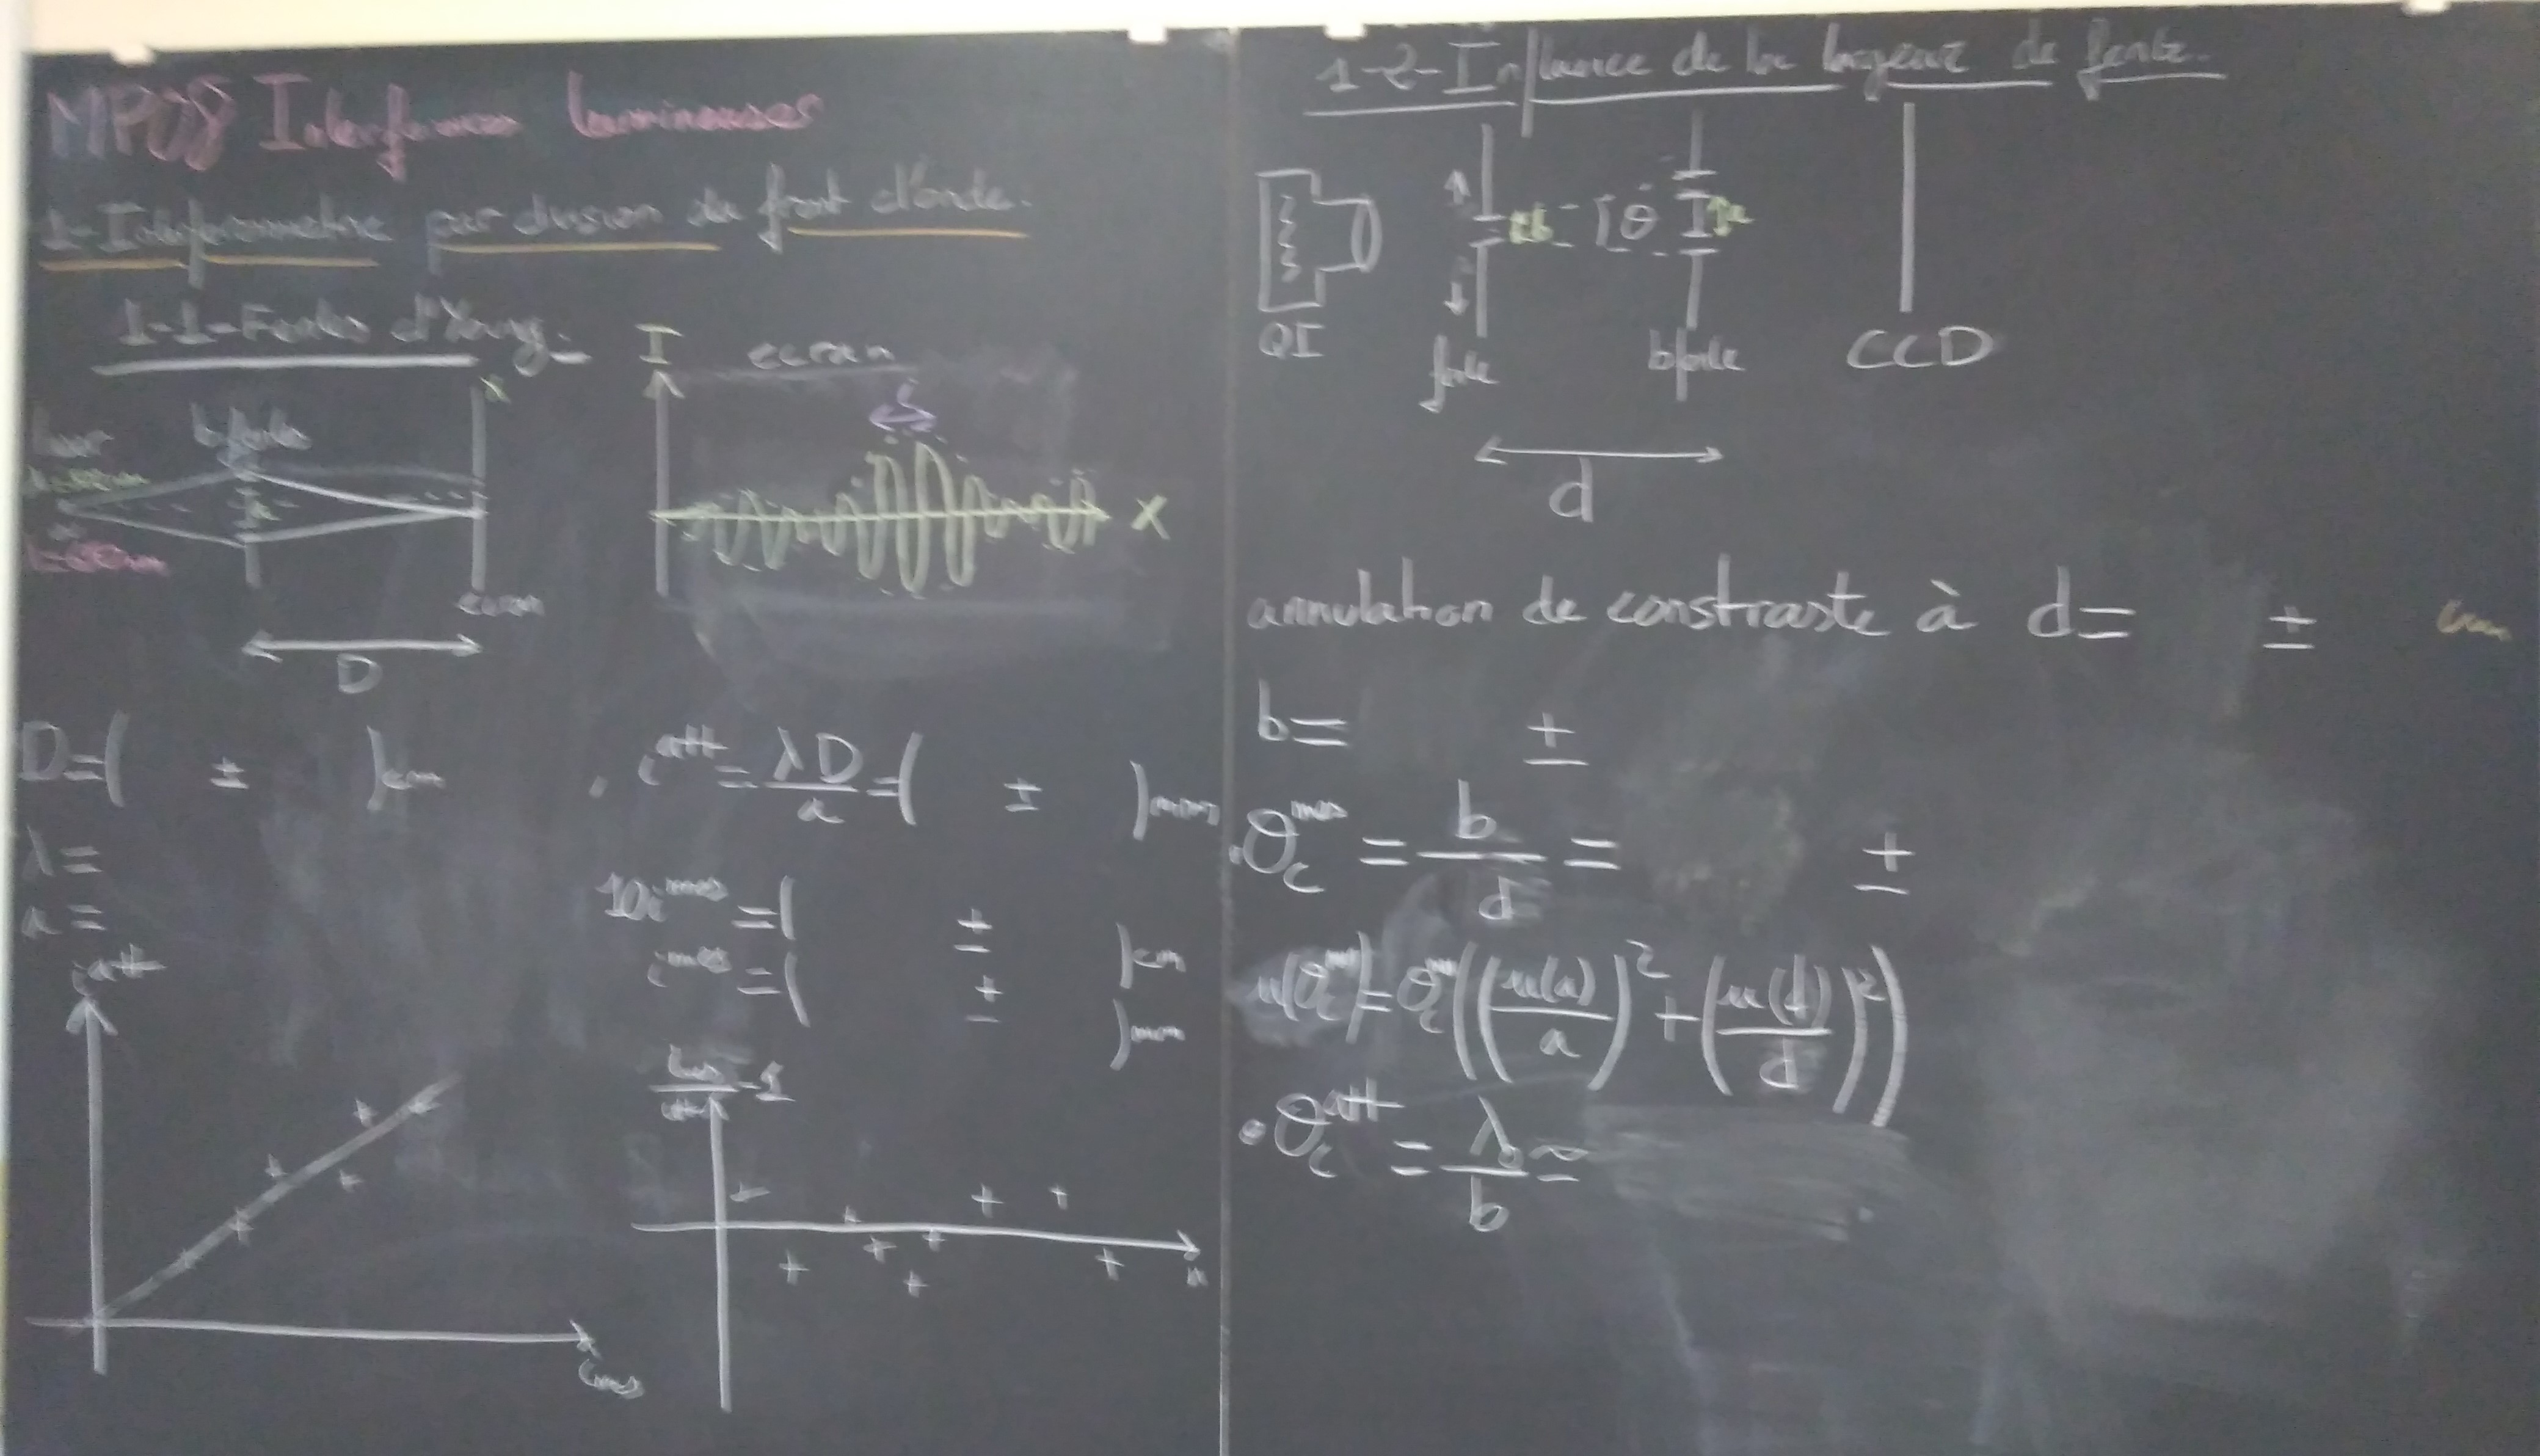
\includegraphics[width=14cm]{p1}}
\end{figure}
	
\section{Interférence par division du front d'onde}
\subsection{Fentes d'Young}
On mesure l'interfrange sur la figure d'interférence formée sur un écran en aval d'une bifente éclairée par un laser. On a en théorie $i = \lambda D/a$, où on mesure D à l'aide d'une ficelle, $\lambda$ peut être mesurée au spectromètre, et où $a$, l'épaisseur des fentes, nous est donnée par le constructeur (peut être obtenu avec une lentille convergente et une mire). Pour la mesure de $i$ on relève la position $x_n$ des extinctions et on trace $x_n(n)$, avant de le modéliser par une droite, on a alors $i$ donné par le coefficient directeur de la droite obtenue.

\subsection{Influence de la largeur de la fente/ cohérence spatiale}
On a cette fois une bi-fente de largeur ajustable qui est éclairée par une fente, et on observe la netteté de la figure d'interférence sur un écran. Pour plus de précision on remplace l'écran par une barrette CCD, on voit alors que lorsque la fente s'ouvre les maximas d'intensité se rapprochent jusqu'à ce que l'on ne puisse plus les distinguer.\\
Justifier le fait d'ouvrir la fente par le fait que la figure étant peu nette on veut plus de lumière.\\
On peut alors estimer \\

Pour quelle valeur de $d$, la distance entre la fente et la bi-fente, et,\\

Pour quelle valeur de $b$\\
On perd le contraste.\\

On obtient alors, en notant $b$ l'épaisseur de la fente 
\begin{eqnarray}
\theta_{max} = \frac{b}{d}
\end{eqnarray}
que l'on peut comparer à 
\begin{eqnarray}
\theta_{max}^{att} =\frac{\lambda}{b}
\end{eqnarray}

\section{Interférence par division d'amplitude}
\begin{figure}
	\centerline{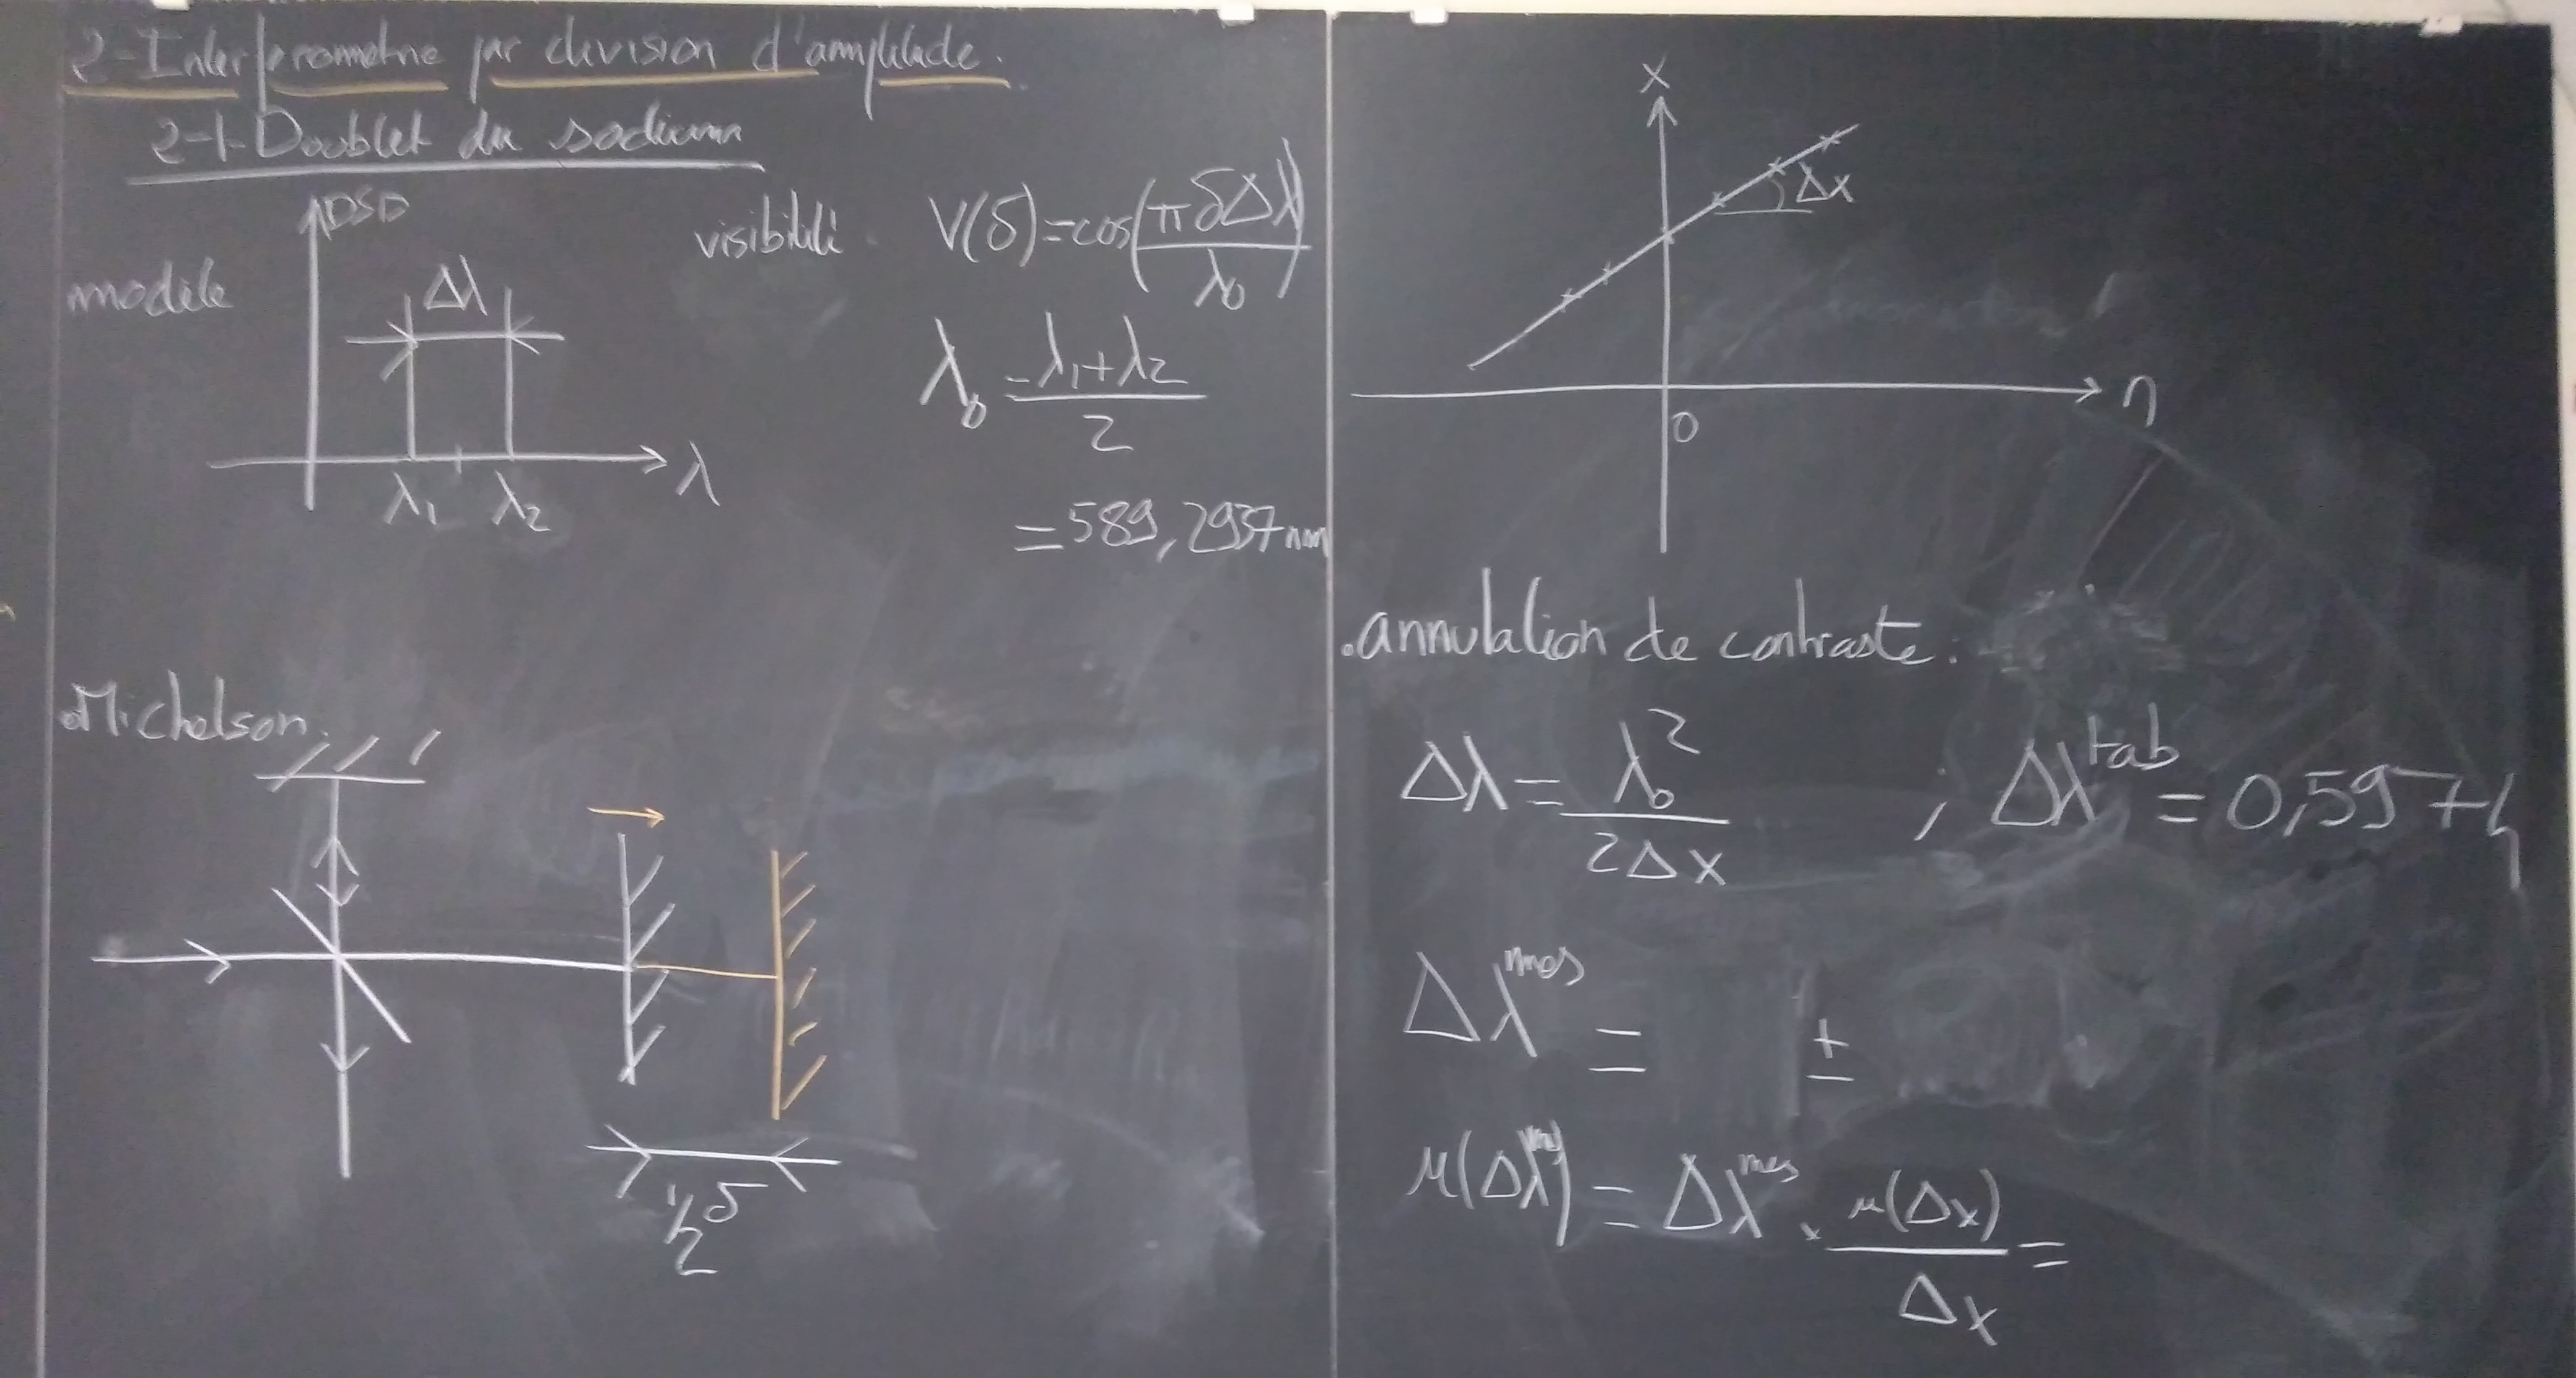
\includegraphics[width=14cm]{p2}}
\end{figure}
\subsection{Doublet du sodium/ cohérence temporelle}
On va résoudre le doublet du sodium à l'aide d'un interféromètre de Michelson réglé en lames parallèles. On a comme visibilité
\begin{eqnarray}
V(\delta) = \cos\left(\frac{\pi\delta \Delta\lambda}{\lambda_0^2}\right)
\end{eqnarray}
avec $\frac{\delta}{2}$ l'écart (en terme de différence de marche) entre les deux miroirs.\\
Là encore on repère les positions $x_n$ des annulations de contraste, en regardant la position $x_n^1$  où on commence à perdre le contraste et $x_n^2$ où le contraste réapparait, et en prenant donc $x_n = \frac{x_n^1+x_n^2}{2}$. On trace alors $x_n(n)$ avant de modéliser par une droite pour obtenir un coefficient directeur $\Delta x$. On a alors 
\begin{eqnarray}
\Delta \lambda = \frac{\lambda_0^2}{2\Delta x}
\end{eqnarray}

\section*{Questions}
Peut on améliorer le résultat de la deuxième manip (ou on éclaire en lumière blanche) ?\\
En utilisant un filtre.\\

Comment fonctionne le filtre sur la paillasse ?\\
Filtre interférentiel.\\

Où faut il placer le filtre ?\\
Devant la CCD pour limiter dans un même temps le bruit.\\

Dans quel domaine la lampe émet elle majoritairement ?\\
Filament de tungstène : 1,5-2 $\mu m$.\\

La barrette CCD est elle sensible dans ce domaine ? Peut on alors utiliser un filtre IR ?\\

Quel type d'incertitude a t'on pour la première manip ?\\
Type B : incertitudes de mesures. \\

Comment faut il alors estimer l'incertitude de lecture lorsqu'on mesure les $x_n$ à la règle après le pointé ?\\
C'est une incertitude de type triangulaire, on a donc une incertitude de $1/\sqrt{6}$ mm.\\

Comment savoir au regard des résidus si les incertitudes évaluées sont correctes ?\\
On regarde la dispersion des points et le rapport entre le $\sigma$ correspondant et l'incertitude évaluée doit être proche de 1.\\

Quelle est le rôle du condenseur ?\\
Le condenseur a pour but de s'assurer que l'on fait bien travailler la lentille (ou le miroir sphérique) dans les conditions de Gauss. Il permet aussi d'avoir plus de lumière.\\

Dans le cas du Michelson, à quoi sert la lentille en sortie ? Et où doit on passer l'écran par rapport à elle ?\\

Q'entendez vous pour le doublet du sodium, q'on "modélise le doublet par deux pics de Dirac" ?\\

Que se passe t'il (pour la visibilité) si on remplace les Dirac par leur allure réelles ?\\
On a non plus un cosinus mais un cosinus amorti qui tend vers 0 en + et -$\infty$ : on a une extension spatiale finie.\\

A quoi ressemble la densité spectrale en réalité ?\\
On a des gaussienne ou presque, a cause des collisions, de l'effet Doppler.\\

Pour la seconde manip, a quoi correspond $\lambda$ puisqu'on éclaire en lumière blanche ?\\

Etes vous dans les conditions de Fraunhoffer ?\\
Il faut regarder si l'inverse du nombre de Fresnel $\frac{\lambda D}{a^2}$ est grand devant 1.



\section*{Remarques}
Il faut évoquer Fraunhoffer.\\
On peut ajouter une mesure de la longueur d'onde du laser au spectro USB, en étalonnant (pour le laser rouge) avec les raies rouges de l'helium ey de l'hydrogène qui tombent de part et d'autre.\\
Il faut explicitement parler de cohérence temporelle et de cohérence spatiale.
	
\end{document}